% Options for packages loaded elsewhere
\PassOptionsToPackage{unicode}{hyperref}
\PassOptionsToPackage{hyphens}{url}
\PassOptionsToPackage{dvipsnames,svgnames,x11names}{xcolor}
%
\documentclass[
  10pt,
]{article}
\usepackage{amsmath,amssymb}
\usepackage{iftex}
\ifPDFTeX
  \usepackage[T1]{fontenc}
  \usepackage[utf8]{inputenc}
  \usepackage{textcomp} % provide euro and other symbols
\else % if luatex or xetex
  \usepackage{unicode-math} % this also loads fontspec
  \defaultfontfeatures{Scale=MatchLowercase}
  \defaultfontfeatures[\rmfamily]{Ligatures=TeX,Scale=1}
\fi
\usepackage{lmodern}
\ifPDFTeX\else
  % xetex/luatex font selection
  \setmainfont[]{DejaVu Serif}
  \setmonofont[]{DejaVu Sans Mono}
\fi
% Use upquote if available, for straight quotes in verbatim environments
\IfFileExists{upquote.sty}{\usepackage{upquote}}{}
\IfFileExists{microtype.sty}{% use microtype if available
  \usepackage[]{microtype}
  \UseMicrotypeSet[protrusion]{basicmath} % disable protrusion for tt fonts
}{}
\makeatletter
\@ifundefined{KOMAClassName}{% if non-KOMA class
  \IfFileExists{parskip.sty}{%
    \usepackage{parskip}
  }{% else
    \setlength{\parindent}{0pt}
    \setlength{\parskip}{6pt plus 2pt minus 1pt}}
}{% if KOMA class
  \KOMAoptions{parskip=half}}
\makeatother
\usepackage{xcolor}
\usepackage[margin=18mm]{geometry}
\usepackage{longtable,booktabs,array}
\usepackage{calc} % for calculating minipage widths
% Correct order of tables after \paragraph or \subparagraph
\usepackage{etoolbox}
\makeatletter
\patchcmd\longtable{\par}{\if@noskipsec\mbox{}\fi\par}{}{}
\makeatother
% Allow footnotes in longtable head/foot
\IfFileExists{footnotehyper.sty}{\usepackage{footnotehyper}}{\usepackage{footnote}}
\makesavenoteenv{longtable}
\usepackage{graphicx}
\makeatletter
\def\maxwidth{\ifdim\Gin@nat@width>\linewidth\linewidth\else\Gin@nat@width\fi}
\def\maxheight{\ifdim\Gin@nat@height>\textheight\textheight\else\Gin@nat@height\fi}
\makeatother
% Scale images if necessary, so that they will not overflow the page
% margins by default, and it is still possible to overwrite the defaults
% using explicit options in \includegraphics[width, height, ...]{}
\setkeys{Gin}{width=\maxwidth,height=\maxheight,keepaspectratio}
% Set default figure placement to htbp
\makeatletter
\def\fps@figure{htbp}
\makeatother
\setlength{\emergencystretch}{3em} % prevent overfull lines
\providecommand{\tightlist}{%
  \setlength{\itemsep}{0pt}\setlength{\parskip}{0pt}}
\setcounter{secnumdepth}{-\maxdimen} % remove section numbering
\ifLuaTeX
  \usepackage{selnolig}  % disable illegal ligatures
\fi
\usepackage{bookmark}
\IfFileExists{xurl.sty}{\usepackage{xurl}}{} % add URL line breaks if available
\urlstyle{same}
\hypersetup{
  colorlinks=true,
  linkcolor={Maroon},
  filecolor={Maroon},
  citecolor={Blue},
  urlcolor={Blue},
  pdfcreator={LaTeX via pandoc}}

\author{}
\date{}

\begin{document}

\section{Target recovery with matched endomorphism
equations}\label{target-recovery-with-matched-endomorphism-equations}

The fixed 42-configuration panel has independently verified native/PARI
results. Twenty-nine bases fill; thirteen remain underfilled. Of 252
planned matrix cases, 174 are analyzed and 78 are excluded by the
predeclared underfill rule. Adding known endomorphism equations resolves
14 previously ambiguous cases. Ordinary bases benefit as well as
twist-derived bases. This is one public toy DLP with correlated matrix
cases, not 114 independently recovered targets or a cost result.

\begin{longtable}[]{@{}
  >{\raggedright\arraybackslash}p{(\columnwidth - 8\tabcolsep) * \real{0.2000}}
  >{\raggedleft\arraybackslash}p{(\columnwidth - 8\tabcolsep) * \real{0.2000}}
  >{\raggedleft\arraybackslash}p{(\columnwidth - 8\tabcolsep) * \real{0.2000}}
  >{\raggedleft\arraybackslash}p{(\columnwidth - 8\tabcolsep) * \real{0.2000}}
  >{\raggedleft\arraybackslash}p{(\columnwidth - 8\tabcolsep) * \real{0.2000}}@{}}
\toprule\noalign{}
\begin{minipage}[b]{\linewidth}\raggedright
Base rule and transform
\end{minipage} & \begin{minipage}[b]{\linewidth}\raggedleft
Analyzed off/on pairs
\end{minipage} & \begin{minipage}[b]{\linewidth}\raggedleft
Target fixed, off
\end{minipage} & \begin{minipage}[b]{\linewidth}\raggedleft
Target fixed, on
\end{minipage} & \begin{minipage}[b]{\linewidth}\raggedleft
Newly fixed
\end{minipage} \\
\midrule\noalign{}
\endhead
\bottomrule\noalign{}
\endlastfoot
Curve progression, half seeds plus alpha images & 15 & 8 & 13 & 5 \\
Curve progression, plain & 18 & 12 & 12 & 0 \\
Ascending x, half seeds plus alpha images & 9 & 6 & 8 & 2 \\
Ascending x, plain & 9 & 6 & 6 & 0 \\
Maximal-seed twist progression, half seeds plus alpha images & 18 & 10 &
16 & 6 \\
Maximal-seed twist progression, plain & 18 & 8 & 9 & 1 \\
\end{longtable}

These are recorded exact counts from
\texttt{execution-v14/SUMMARY.json}. The 14-case change is the sum of
its newly-fixed counts, \(5+2+6+1\). Unequal denominators, overlapping
arity modes and reused target forbid treating this table as a population
success-rate comparison. The first-seed twist rules are absent from the
filled table because all twelve underfill; their full records remain.

\begin{figure}
\centering
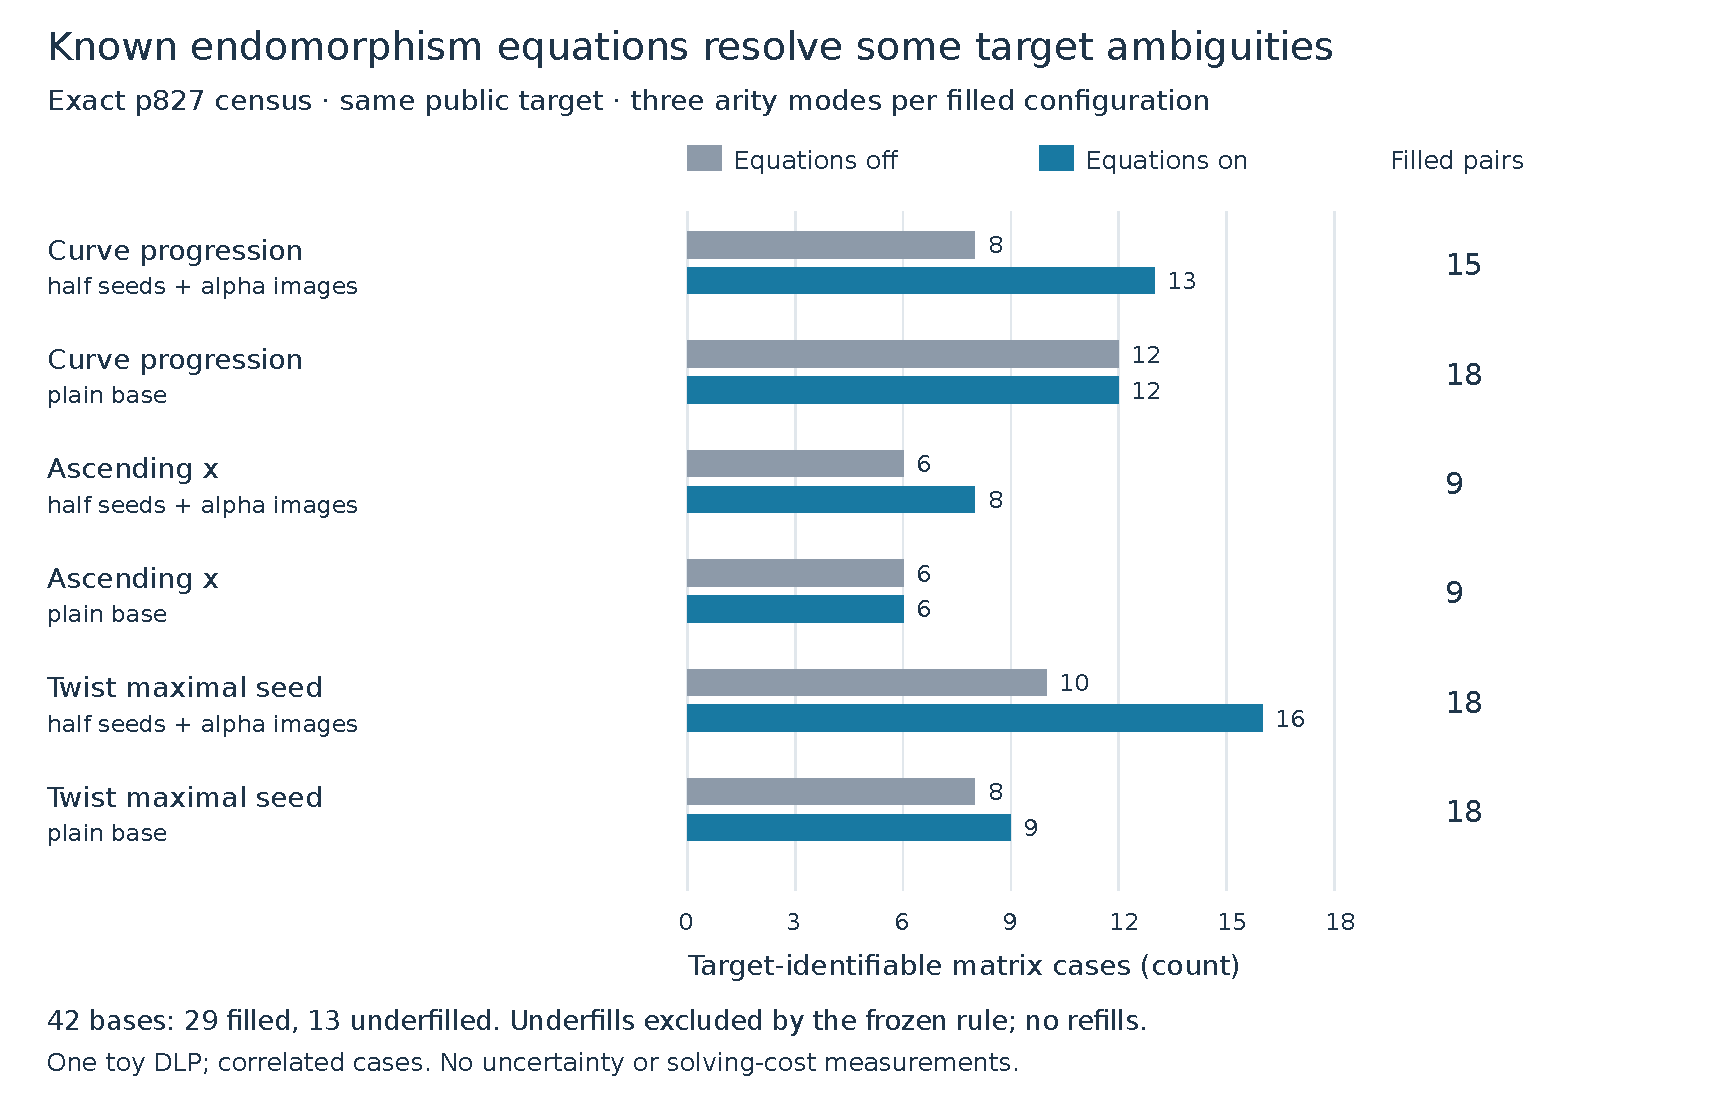
\includegraphics{IDENTIFIABILITY.pdf}
\caption{Recorded target-identifiability counts with known alpha
equations off/on. Native run rank-v1 and independent GP run pari-v1,
protocol v14. Counts are a complete finite census; no sampling
uncertainty or clocks are admitted.}
\end{figure}

\subsection{Exact task and controls}\label{exact-task-and-controls}

The unchanged source is \(E:y^2=x^3+x+15\) over \(\mathbb F_{827}\),
order823, \(G=(2,5)\), ICV1 \texttt{icv1-fp10-t5-192cb216}; public
\(Q=[37]G\). Its rational twist is \(T:Y^2=X^3+4X+120\), order833, group
\(C_7\times C_{119}\). The given first seed \((0,51)\) has order7 and
maximal seed \((2,386)\) has order119. The certified degree17 map
\(\alpha=(\pi+[1])/[7]\) acts as353 on \(E(\mathbb F_{827})\). Map
discovery was an input to this diagnostic and is not charged here.

For each B8/12/16, seven fixed rules use ascending x, curve progressions
at shifts1/3, and first/maximal twist progressions at shifts1/3. Orbit
coordinates are lifted on the original curve after the fixed shift;
twist X is divided by2 first. G anchors each base. The plain transform
requests B seed points; the other requests B/2 and unions them with
canonical alpha images. There is no post-outcome refill, replacement,
truncation or base selection using Q or its log.

All ordinary and twist bases receive the same map checks and known
scalar information. Internal canonical edges give
\(u_j-c u_i=0\pmod{823}\) with \(c=353\) or \(-353\), depending on
orientation. Compare these equations off/on. An internal edge is known
information, not a newly sampled query relation.

Every filled base collects all signed two-/three-term witnesses for
\(Q+[j]G\), \(j=0,\ldots,15\), including repetitions and multiplicities.
Each base has arity2, arity3 and their union, crossed with equations
off/on. The single native execution retains 928 attempted queries, 402
zero-witness queries and 5389 raw witnesses. The remaining planned
queries were not attempted on underfills. All395 base-point map/scalar
controls pass, including rejection of scalar354. Two archived bases and
all64 corresponding query witness sets match v8 exactly.

All twelve first-seed twist configurations underfill: their final sizes
are 3/6 for shift1 plain/augmented and1/2 for shift3. The remaining
underfill is B16 curve-shift1 augmented, final size15 after a collision.
All13 records and their78 excluded matrix cells are explicit. No extra
queries were sampled.

\subsection{What changed, and what stayed
ambiguous}\label{what-changed-and-what-stayed-ambiguous}

The archived B8 maximal-twist shift1 plain base still gives66 raw
witnesses, 15 distinct equations, rank8 in9 unknowns, and an ambiguous
target. It has no internal alpha edge, so enabling the equations changes
nothing.

For B8 maximal-twist shift3 with half seeds plus alpha images, arity3
gives 19 raw witnesses and8 distinct query equations. Known equations
raise rank6 to9 in9 unknowns and determine the public target scalar37.
This verifies one modified twist-derived base that resolves the earlier
type of ambiguity; it does not repair the original base or prove a
twist-specific mechanism.

The ordinary B8 curve-shift3 augmented base gives an informative
counterpoint: arity2 has3 distinct query equations; adding known
equations raises rank3 to7 in9 unknowns, and the target is fixed
although other unknown logs remain free. The maximal-twist B16 shift1
plain arity2 case also fixes the target at rank12 in17 unknowns. Thus
full column rank is sufficient but unnecessary for recovery.

The analysis keeps the rank of anchor/alpha equations separate from the
new rank contributed by query equations. It does not credit known scalar
edges as independent sampled relations. Across all174 analyzed cells,
114 fix the target and60 leave it ambiguous; every fixed scalar passes
the original public point check. Every ambiguous case includes two
distinct target coordinates satisfying every equation. The eliminator
receives no factor-base log table or scalar37.

\subsection{Independent and formal
verification}\label{independent-and-formal-verification}

For \(Mx=b\), a particular solution \(x_0\) and a complete kernel basis
describe the affine fiber \(x_0+\ker M\). The target coordinate is fixed
exactly when its projection vanishes on the whole kernel. Native exact
RREF records this fiber, not just rank. PARI independently rebuilds
every base and alpha map using \texttt{ellisogeny}, every edge, witness,
deduplicated equation, rank, kernel dimension and span, particular
solution, target projection and recovery/ambiguity check.

Both scientific processes complete successfully. Strict admission checks
process status, all script/output hashes, sole marker
\texttt{ALL\_TWIST\_RANK\_REPAIR\_OK\ 42}, and empty stderr or only the
predeclared GP stack-size warning. The combined export has
planned2/attempted2/completed2/interrupted0/resumed0/excluded0
processes. Base underfills are within-run exclusions, not missing
process rows.

Lean declarations
\texttt{TwistTargetIdentifiability.target\_fiber\_iff\_kernel} and
\texttt{kernel\_witness\_changes\_target} prove the general
additive-homomorphism fiber criterion and an explicit ambiguity witness.
Lean4.34.1, pinned mathlib
\texttt{d13f23b7\allowbreak{}23b8a846\allowbreak{}827a245b\allowbreak{}89c10fc7\allowbreak{}d3f11612}, frozen build and
fresh native transitive axiom audit pass for both theorems, standard
foundations only. The concrete finite matrix, field, complete kernel
basis and elliptic-curve extraction bridge remain outside these formal
proofs. This is not a formally checked proof of every concrete matrix.
No characteristic827 symbolic identity is being promoted through the
fixed-modulus identity-certificate format.

The native diagnostic's19 tests and full standalone runner package pass.
Before freeze, synthetic F101 controls exposed two GP matrix-shape
defects; both failed attempts are preserved, followed by a successful
corrected control. The first Lean development import failure is retained
with the successful development/frozen replays. The main panel ran once
with no retry/amendment. The earlier named full-root validation gap
remains open; this package pass does not imply a complete root suite or
CI pass.

\subsection{Pins, reproduction and
scope}\label{pins-reproduction-and-scope}

Source \texttt{d3772516\allowbreak{}11bc9fd3\allowbreak{}da22096c\allowbreak{}3b128862\allowbreak{}816ef268}; committed
freeze before data; protocol hash
\texttt{e031cee9\allowbreak{}1eef30ca\allowbreak{}50d2ddef\allowbreak{}24cd36c7\allowbreak{}ca6ee739\allowbreak{}a3f173bd\allowbreak{}9885005e\allowbreak{}fb7c61bf}.
Inputs, binaries, commands and caps are in execution-v14 FROZEN/PROTOCOL
files. Native and GP use one thread, CPU0, 4GiB and300s each on the
managed Xeon8573C KVM host, L0, under the recorded EKS image-access
fallback. No clocks, paid allocation or external-tool performance
comparison is claimed. The controls use independent implementations on
the same host/author, not independent review.

Raw archive:61888bytes/ten files, SHA256
\texttt{2fd7a36e\allowbreak{}7a9755ea\allowbreak{}9687e93d\allowbreak{}7cc86bec\allowbreak{}661943dc\allowbreak{}f6fb6385\allowbreak{}3968432b\allowbreak{}52d41e13}.
It is in the user-confirmed
\texttt{s3://setec-astronomy-artifacts/store}; publication verification
records the fresh download, all member hashes and deterministic repack
separately. See \href{../../execution-v14/README.md}{execution-v14} for
commands, the complete42/252-cell records, unified export and exact
validation receipts.

Literature reviewed before implementation: repository factor-base/GLV
synthesis, v8/v9 rank evidence and v10 map construction; primary
MIT18.783 Fall2025
\href{https://math.mit.edu/classes/18.783/2025/LectureNotes13.pdf}{Lecture13},
Theorems13.6/13.8; official
\href{https://pari.math.u-bordeaux.fr/dochtml/html-stable/Vectors__matrices__linear_algebra_and_sets.html}{PARI
matrix documentation} and installed help for \texttt{matker},
\texttt{matrank}, \texttt{matinverseimage}. Affine-kernel linear algebra
and endomorphism scalar equations are standard methods.

This completes the bounded relation-repair diagnostic in its filed card,
including the matched augmentation extension. It leaves the separately
frozen complete cold-cost panel, strongest ordinary/group/external
controls, larger held-out curves, original E00--E29 campaigns and
concrete formal bridges open. The result provides no novelty, IC
speedup, asymptotic or NIST conclusion. Canonical progress timeline, IC
scoreboard, curve diagrams and performance charts were checked: no
model/map or admitted cost value changes, so those graphs are unchanged.
The new quantitative graph records this diagnostic only.

\end{document}
